\documentclass[xcolor=table]{llncs}
\usepackage{booktabs}
\usepackage[table,xcdraw]{xcolor}
\usepackage[pdftex]{graphicx}  
\begin{document}
\title{Assigment 3 - Is it on cache?}
\author{Marco Espinoza \newline Jose Campos}
\institute{Instituto Tecnológico de Costa Rica}
\maketitle
\section{First reference misses}
The program main.c was executed 4 times using the program perf stat to track the number of cache references and cache misses during our main program execution. 
The results obtained are the following:
\begin{center}
\begin{table}[]
\centering
\caption{Perf stat results after 4 main program executions}
\label{table1}
\begin{tabular}{ccccccc}
\hline
\rowcolor[HTML]{000000} 
{\color[HTML]{FFFFFF} \textbf{\#}} & {\color[HTML]{FFFFFF} \textbf{\begin{tabular}[c]{@{}c@{}}Time elapsed \\ (ms)\end{tabular}}} & {\color[HTML]{FFFFFF} \textbf{\begin{tabular}[c]{@{}c@{}}Task-clock \\ (msec)\end{tabular}}} & {\color[HTML]{FFFFFF} \textbf{cycles}} & {\color[HTML]{FFFFFF} \textbf{instructions}} & {\color[HTML]{FFFFFF} \textbf{cache-references}} & {\color[HTML]{FFFFFF} \textbf{cache-misses}} \\ \hline
1 & 10,909 & 0,267 & 630722 & 423164 & 22265 & 10477 \\
2 & 0,446 & 0,202 & 595425 & 420416 & 22047 & 5813 \\
3 & 0,389 & 0,192 & 529091 & 426025 & 23513 & 2800 \\
4 & 0,487 & 0,223 & 517475 & 425037 & 21689 & 1907 \\ \hline
\end{tabular}
\end{table}
\end{center}
%
\subsection{Questions}
%
a. Why did the first run of your application report a high cache miss rate?\newline
Because during the first execution, the program is stored in the hard drive, and it is not loaded in the main memory or in the L2 cache.
It produces the program must to be moved from the drive to the cache, and it produces misses during the program execution.\newline\newline
b. Why did any subsequent execution report a decremental cache miss rate?\newline
Because after the first execution, multiples sections of the program is stored in the L2 cache, and it produces hits during the second and the next program executions. Additionally, due to the locality of reference, the number of misses is reduced.\newline
Those locality of reference consists on temporal and spacial locality, where the temporal locality refers to the reuse of specific data, and/or resources, within a relatively small time duration. Spatial locality refers to the use of data elements within relatively close storage locations memory.\newline
For those reasons the number of cache miss rate is reduced after the subsequent program execution.
\newline
%
\section{Optimizing memory accesses on loops}
%
On this section, the main application located into the part\_2 directory of the project files was used to be compiled through 2 kind of memory ordering, row and columns. 
The program was executed using both methods 5 times using perf stat to compare both results in terms of cache memory access. The results will be exposed in the following sections.\newline
\subsection{Row results}
The results obtained for the row results are presented in the next table.
\begin{table}[]
\centering
\caption{Perf stat results using row ordering during 5 times}
\label{table2}
\begin{tabular}{ccccccc}
\hline
\rowcolor[HTML]{000000} 
{\color[HTML]{FFFFFF} \textbf{\#}} & {\color[HTML]{FFFFFF} \textbf{\begin{tabular}[c]{@{}c@{}}Time elapsed \\ (ms)\end{tabular}}} & {\color[HTML]{FFFFFF} \textbf{\begin{tabular}[c]{@{}c@{}}Task-clock \\ (msec)\end{tabular}}} & {\color[HTML]{FFFFFF} \textbf{cycles}} & {\color[HTML]{FFFFFF} \textbf{instructions}} & {\color[HTML]{FFFFFF} \textbf{cache-references}} & {\color[HTML]{FFFFFF} \textbf{cache-misses}} \\ \hline
1                                  & 134.57                                                                                       & 4.583                                                                                        & 11628737                               & 24742637                                     & 202382                                           & 121747                                       \\
2                                  & 4.174                                                                                        & 3.894                                                                                        & 10964320                               & 24591759                                     & 150668                                           & 59725                                        \\
3                                  & 7.578                                                                                        & 7.061                                                                                        & 11608162                               & 24534858                                     & 153962                                           & 86481                                        \\
4                                  & 27.237                                                                                       & 4.173                                                                                        & 11261520                               & 24515829                                     & 148946                                           & 77911                                        \\
5                                  & 15.436                                                                                       & 3.953                                                                                        & 11056268                               & 24542301                                     & 155608                                           & 76989                                        \\ \hline
\end{tabular}
\end{table}\newline\newline
\subsection{Column results}
The results obtained for the column results are presented in the table 3.
\begin{table}[]
\centering
\caption{Perf stat results using row ordering during 5 times}
\label{table3}
\begin{tabular}{ccccccc}
\hline
\rowcolor[HTML]{000000} 
{\color[HTML]{FFFFFF} \textbf{\#}} & {\color[HTML]{FFFFFF} \textbf{\begin{tabular}[c]{@{}c@{}}Time elapsed \\ (ms)\end{tabular}}} & {\color[HTML]{FFFFFF} \textbf{\begin{tabular}[c]{@{}c@{}}Task-clock \\ (msec)\end{tabular}}} & {\color[HTML]{FFFFFF} \textbf{cycles}} & {\color[HTML]{FFFFFF} \textbf{instructions}} & {\color[HTML]{FFFFFF} \textbf{cache-references}} & {\color[HTML]{FFFFFF} \textbf{cache-misses}} \\ \hline
1                                  & 57.02                                                                                        & 5.117                                                                                        & 13173982                               & 24687156                                     & 258039                                           & 122711                                       \\
2                                  & 4.549                                                                                        & 4.25                                                                                         & 12371551                               & 24591174                                     & 206147                                           & 59734                                        \\
3                                  & 35.83                                                                                        & 4.42                                                                                         & 12422663                               & 24580902                                     & 212715                                           & 79864                                        \\
4                                  & 17.95                                                                                        & 4.803                                                                                        & 13089132                               & 24571754                                     & 237982                                           & 85326                                        \\
\multicolumn{1}{l}{5}              & 21.60                                                                                        & 4.45                                                                                         & 12696407                               & 24502248                                     & 232095                                           & 78962                                        \\ \hline
\end{tabular}
\end{table}
\subsection{Questions}
\paragraph{}
a. What kind of optimization is performed on the program?\newline
The kind of optimization performed on the program is called permutation. Loop permutation takes advantage of the memory ordering used by an specific programming language for data allocation improving data locality. The followed image present both examples used on this section, row and column ordering.\newline
\begin{figure}
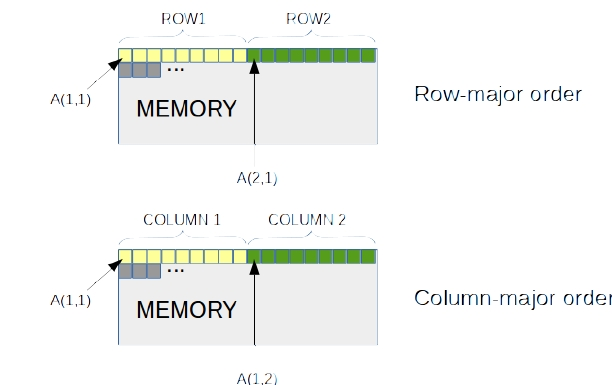
\includegraphics[scale=0.4]{row_column.jpg}
\centering
\caption{Figure1}
\label{fig: Row and Column ordering implemented in the section 2}
\end{figure}\newline
\paragraph{}
b. Why does the cache miss rate is higher for the row results? Is this expected according to the loop optimizations implemented? Provide detail on your thoughts.\newline
\paragraph{}
As it is showed in the figure 1, the row major schema consists on try to store the row data into the same cache line. It produces, during each row iteration the same cache line is accessed, allowing to keep the program in the MLC (Mid Level Cache). It reduces the number of cache references tracked by the perf stat program, because it is checking the LLC and not the MLC.\newline
Due to C implement row major scheme, the miss rate is higher for the row results, because the number of cache references is lower in the LLC. This is expected for this kind of optimization, due to as it was explained, the program will be most of the time in the MLC, increasing the miss rate due to only the LLC is taked into account by the perf stat program.
The next table presents the miss-rate for both orderings.
\begin{table}[]
\centering
\caption{Row miss rate vs Column miss rate}
\label{table4}
\begin{tabular}{ccc}
\hline
\rowcolor[HTML]{000000} 
{\color[HTML]{FFFFFF} \textbf{\#}} & {\color[HTML]{FFFFFF} \textbf{Column Miss Rate}} & {\color[HTML]{FFFFFF} \textbf{Row Miss Rate}} \\ \hline
1                                  & 47.555\%                                         & 60.157\%                                      \\
2                                  & 28.976\%                                         & 39.640\%                                      \\
3                                  & 37.545\%                                         & 56.170\%                                      \\
4                                  & 35.854\%                                         & 52.308\%                                      \\
\multicolumn{1}{l}{5}              & 34.022\%                                         & 49.476\%                                      \\ \hline
\end{tabular}
\end{table}
\newline
\newline
\newline
\paragraph{}
c. Why do the cache references are higher for the column results? Provide detail on your thoughts.\newline
As it was explained in the answer b, C uses row major schema, and it produces during each column iteration, a different cache line is accessed. It increments the probability of misses in the MLC and at the same time increments the number of references to the LLC. 
For this reason, the number of cache references is higher in the column results, because there are misses not tracked by the perf stat program in the MLC, but they are tracked as cache references in the LLC.
The following table shows the results for the cache references obtained in both methods. 
\begin{table}[]
\centering
\caption{Column cache references between Row cache references}
\label{table5}
\begin{tabular}{ccc}
\hline
\rowcolor[HTML]{000000} 
{\color[HTML]{FFFFFF} \textbf{\#}} & {\color[HTML]{FFFFFF} \textbf{Column Cache-References}} & {\color[HTML]{FFFFFF} \textbf{Row Cache References}} \\ \hline
1 & 258039 & 202382 \\
2 & 206147 & 150668 \\
3 & 212715 & 153962 \\
4 & 237982 & 148946 \\
5 & 232095 & 155608 \\ \hline
\end{tabular}
\end{table}
\newline
\newline
\paragraph{}
d. Why do the cache misses are similar between both tests? Is this expected according to the loop optimization method implemented? Provide detail on your thoughts.\newline
In the table 2 and table 3 it is possible to see the number of cache misses is similar between both tests. This is expected according to the loop optimization method implemented due to with the row results the number of cache references is lower because there are more hits in the MLC, and the column results showed more cache references because there are more misses in the MLC and it produces more accesses to the LLC. But, when a miss occurs in the LLC for both results, the program need to get the data from the main memory, and perf stat is tracking those misses. It means, despite the row results can have more hits in the MLC, the number of access to the main memory is almost the same for both tests and it is the reason the cache misses is similar.\newline
e. How is the loop optimization related to the instructions per cycle reported for each test case ( insns per cycle) ?\newline
For the row test case the number of instructions per cycle is higher compared with the column test. This is expected, because as it was explained in the other answers, for the row results there are more hits in the MLC, allowing the core to process instructions faster compared with the column results, because in the row test, the core does not need to wait until the data is provided from the LLC, because the data is already in the MLC.
The following table showed the results for both tests related with the instructions per cycle:
\begin{table}[]
\centering
\caption{Instructions per cycle for row and column tests results}
\label{table6}
\begin{tabular}{ccc}
\hline
\rowcolor[HTML]{000000} 
{\color[HTML]{FFFFFF} \textbf{\#}} & {\color[HTML]{FFFFFF} \textbf{Insns per cycle Column test}} & {\color[HTML]{FFFFFF} \textbf{Insns per cycle Row results}} \\ \hline
1                                  & 1.87                                                        & 2.537                                                       \\
2                                  & 1.99                                                        & 2.816                                                       \\
3                                  & 1.98                                                        & 2.11                                                        \\
4                                  & 1.88                                                        & 2.18                                                        \\
\multicolumn{1}{l}{5}              & 1.93                                                        & 2.22                                                        \\ \hline
\end{tabular}
\end{table} 
%
\end{document}
